\documentclass[9pt, oneside]{article}   	% use "amsart" instead of "article" for AMSLaTeX format
\usepackage[left=2cm, right=2cm, top=3cm]{geometry}
\usepackage{cite}
\usepackage[english]{babel}
\usepackage{geometry}                		% See geometry.pdf to learn the layout options. There are lots.
\geometry{letterpaper}                   		% ... or a4paper or a5paper or ... 
\usepackage{graphicx,kantlipsum,setspace}
\usepackage{caption}			% Use pdf, png, jpg, or eps§ with pdflatex; use eps in DVI mode
\captionsetup[table]{font={stretch=1.15}}     %% change 1.2 as you like
\captionsetup[figure]{font={stretch=1.15}} 
\graphicspath{ {images/} }		% TeX will automatically convert eps --> pdf in pdflatex
\PassOptionsToPackage{hyphens}{url}\usepackage{hyperref}
\renewcommand{\UrlFont}{\small\tt}
\usepackage[euler]{textgreek}
\usepackage{verbatim}						
\usepackage{titlesec}
\titlelabel{\thetitle.\quad}
\usepackage{amssymb}
\linespread{1.15}
\usepackage{gensymb}
\usepackage{textcomp}
\usepackage{setspace}
\usepackage[symbol]{footmisc}
\usepackage[version=4]{mhchem}
\usepackage{multicol}
\setlength\columnsep{20pt}
\usepackage{wrapfig}
\setlength{\parindent}{1cm} % Default is 15pt.
\usepackage{oz}


% 2 is subsection, 3 is subsubsection
\setcounter{tocdepth}{3}

\begin{document}
\newpage


\begin{center}
\Large{\textbf{Data Provenance Over Computational Graphs}}
\vspace{1 cm}

\normalsize{}
Alan Ransil

Protocol Labs

alan@protocol.ai

\vspace{1 cm}
Updated \today

\vspace{1 cm}
\Large{\textbf{Abstract}}

\end{center}

\noindent Data-driven decision making requires trusted information from many sources to be combined using versioned procedures. Here, we introduce two protocols which when used together allow end-to-end tracing of data provenance and trust over computational pipelines. The first protocol, Transform.Storage, models compute pipelines as symmetric monoidal categories anchored in content-addressed data types. This allows both reproducible and non-reproducible real-world processes to be described as accessible wiring diagrams. Secondly, the Provenance Protocol uses signatures over data and code to evaluate trust with respect to a community.  While the two protocols may be used independently, together they form a multi-layer system dynamically tracing the flow of trust through complex and multi-party computational processes. We explore applications of this paradigm to real-world use cases.


\begin{multicols}{2}
\setlength{\parskip}{0.1\baselineskip} %Controls vertical space between paragraphs, can re-set line by line
\section{Introduction}

There is a need to establish the end-to-end reasoning behind data driven decisions, and in particular reasoning incorporating data supplied by many parties. Several trends make this need increasingly urgent. First, the trend towards using public and open source data to substantiate decisions increases the utility of expressing these decisions using transparent end-to-end compute pipelines. Second, decisions are increasingly automated with IOT, smart contract and AI subsystems forming parts of the decision making pipeline. Explicitly recording this pipeline is necessary to substantiate trust in the end result. Third, generative AI heightens the need to rigorously track the provenance of data to combat misinformation. Fourth, decisions in critical areas such as environmental sustainability and AI ethics and safety rely on rapidly evolving research which carries an imperative to explicitly lay out methodologies so that they can be reproduced, challenged, improved, and rapidly applied. Fifth, the introduction of more powerful and general zero knowledge systems increases the necessity of tracing decisions end-to-end so that proven claims relying on little revealed information can be put into context.

Here we introduce two protocols that together can be used to model end-to-end decisions as modular compute pipelines, reproduce their results if sufficient information is revealed, establish trust relative to norms determined by user communities, and allow subsequent users to reuse or extend these pipelines without sacrificing verifiability. These protocols model compute pipelines in three layers as shown in figure \ref{layeredDataFig1}. The first protocol, Transform.Storage, represents functions as modular, directional relationships between data types. At the data Asset layer, this defines pipelines as typed datasets on a two-dimensional grid along with functional maps between them. At the Function layer, Transform.Storage represents function definitions coupled with input and output types. The correspondence between these layers is determined by the types of Assets on the lower level and the input and output types of Functions at the middle level. The second protocol, the Provenance Protocol, can be used to apply provenance information to data, functions and pipelines and define bounded trust in each relative to community norms. While the two protocols can be used separately, together they can be used to automatically map the flow of trust evaluated relative to a given Provenance community.

\begin{center}
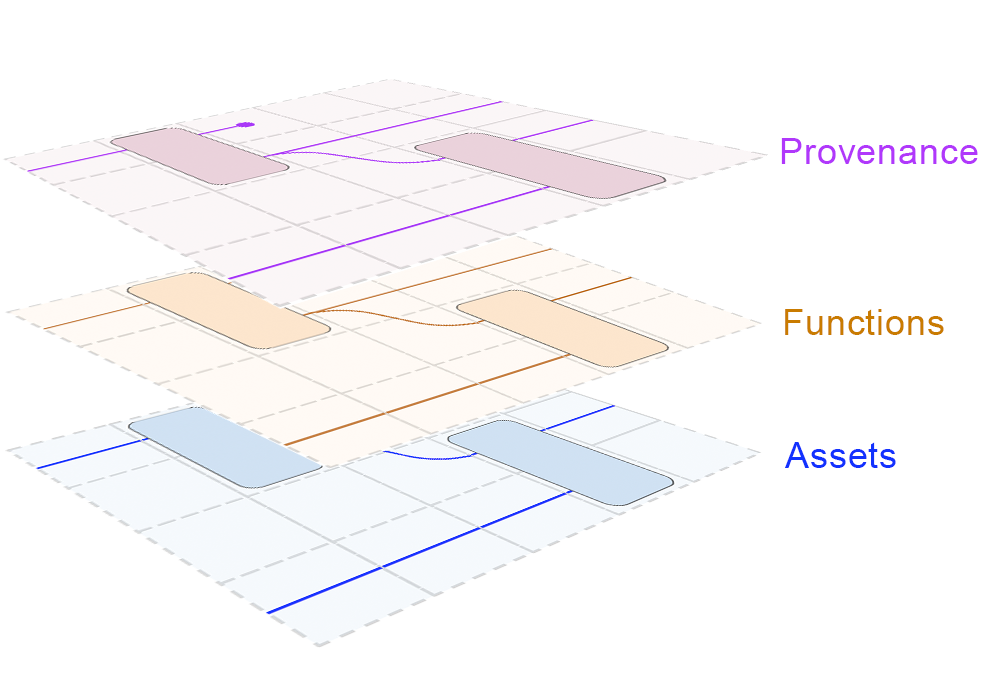
\includegraphics[width=1\columnwidth]{Fig1_assets_20230715}
\begin{flushright}
\captionof{figure}[Three layers of a compute pipeline]{The three layers of a compute pipeline include underlying data assets, functions operating on those assets, and provenance establishing the origins of the lower two layers. Data types establish a correspondence between the asset and function layers, while provenance metadata operating over the lower two layers establishes a flow of trust.}
\label{layeredDataFig1}
\end{flushright}
\end{center}

\section{Previous Work}\label{PrevWork}

This section does not attempt a comprehensive literature review of relevant projects. Included are brief descriptions of some of the work which inspired our approach, highlighting some critical differences in design decisions.

\subsection{Decentralized Identifiers and Verifiable Credentials}\label{did-vc}

The World Wide Web Consortium (W3C) developed standards for Decentralized Identifiers (DIDs) and Verifiable Credentials (VCs) to allow management of identities and credentials without a centralized registry. Following these standards, a self-sovereign DID may be generated for an individual or organization. The DID controller establishes and signs a DID Document which describes the public keys, authentication and delegation protocols, and endpoints associated with the DID. By separating the DID Document from the controller's key pair, this specification enables a persistent self-sovereign identifier that supports method upgrades and key pair rotation. \cite{w3cDID}

\subsection{IPFS}\label{IPFS}
Tracing decisions end-to-end requires interoperating between work done by many individuals on many different computers and subsystems. The protocols typically used to communicate between machines, such as TCP and https, operate on the basis of location addressing. Under this design pattern, information does not have a persistent identifier and interoperability typically relies on centralized services maintaining endpoints which resolve to network locations. Users of these services typically do not control their own key pairs, which disintermediates them from their data. While the results of these design decisions on market power and centralization of economic control are widely discussed, their implications for data management are similarly profound. Because users are expected to rely on companies to maintain the integrity of their data and market incentives induce vendors to lock in users, it is difficult for developers to write code that traces data across the boundaries between software subsystems.

The Interplanetary File System (IPFS) is a protocol which allows users to address and deliver content based on the cryptographic hash of that content rather than its location on the network \cite{ipfs-paper}. This design pattern, namely using a content address as a URI rather than a location address, is essential for maintaining interoperability and will therefore be used as the basis for data addressing in this work.

\end{multicols}
\begin{center}
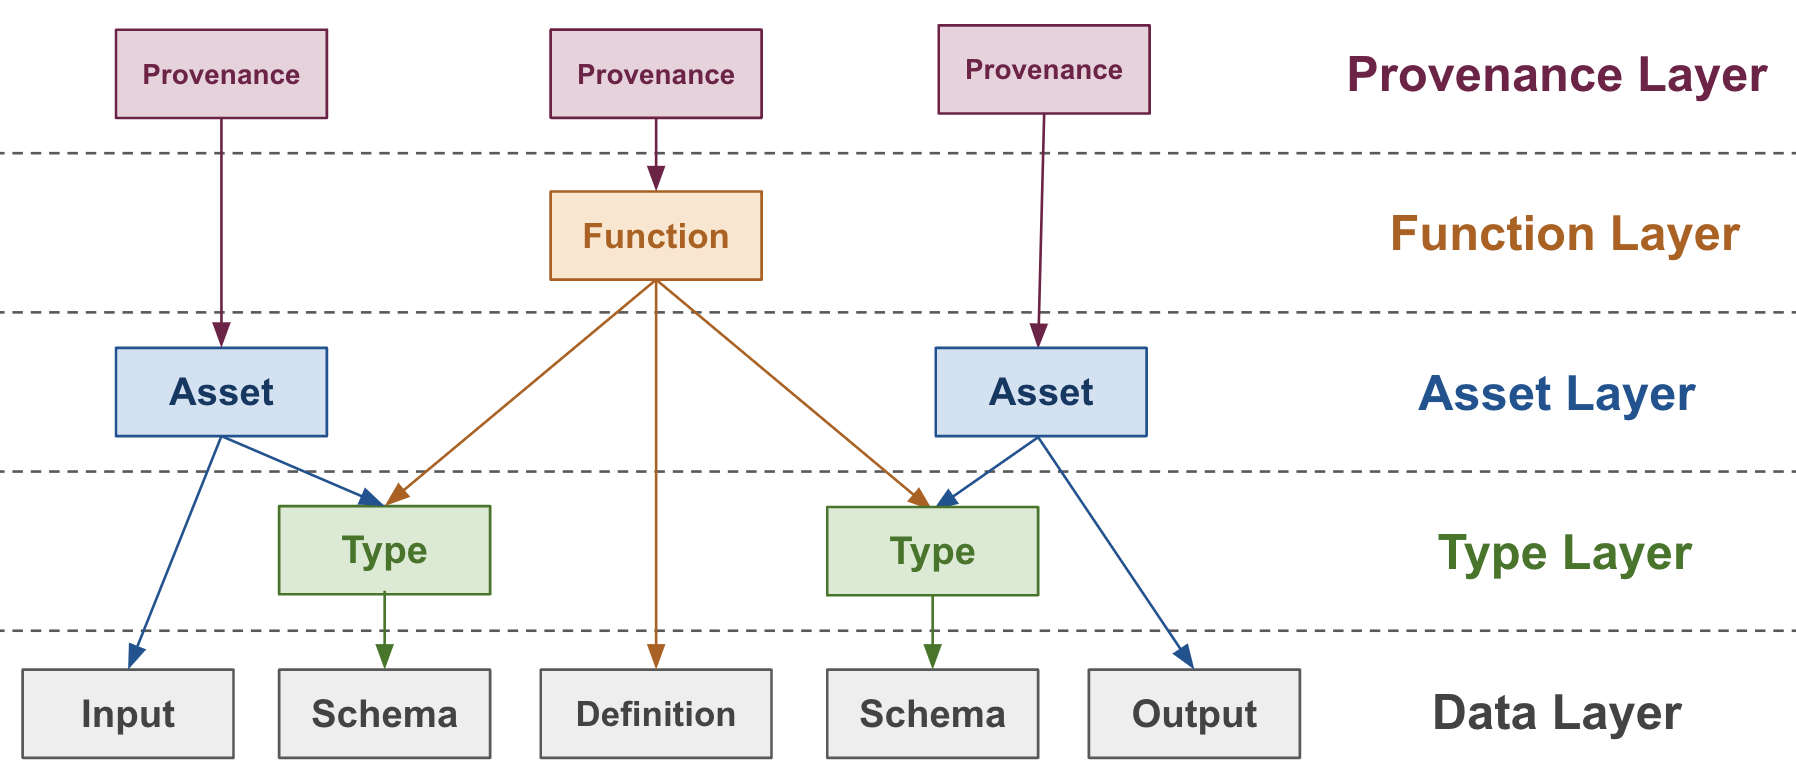
\includegraphics[width=1\columnwidth]{Fig2_layers_20230715}
\begin{flushright}
\captionof{figure}[Simple compute pipeline]{Diagram of a simple compute pipeline consisting of one input asset, one function, and one output asset highlighting relationships between data model components.}
\label{layeredDataFig1}
\end{flushright}
\end{center}
\begin{multicols}{2}


\subsection{Wiring Diagrams and Symmetric Monoidal Categories}\label{smc}

Wiring diagrams are computational graphs in which data types are represented by lines and functions are represented by boxes. It has been shown that they can be interpreted rigorously as representations of symmetric monoidal categories (SMCs). \cite{Patterson_2021} 


A category is a mathematical structure containing objects as well as directional relationships between objects known as morphisms. Morphisms must compose, meaning that if morphisms $f : A \rightarrow B$ (morphism $f$ is a directional relationship from object $A$ to object $B$) and $g : B \rightarrow C$ both exist in a category then there must also exist $h : A \rightarrow C$ such that $h = f \zcmp g$. A monoidal category is a category with a product operation, ie. $(A \otimes B)$. 

A SMC is a monoidal category with a braiding operation $Braid_{A,B} : A \otimes B \rightarrow B \otimes A$ that is symmetric: $Braid_{A,B} \zcmp Braid_{B,A}=Identity_{A \otimes B}$. If objects in a category are interpreted as data types and morphisms as functions mapping from one datatype to another, then the product in an SMC can be interpreted as an ordered set of two non-interacting data types. 

Representing data pipelines in transform.storage as wiring diagrams is provides a formal grounding for computational diagrams that behave intuitively. The type structure makes it possible to define which functions are allowed to be composed with other functions, and by anchoring types using content addresses we are able to achieve interoperability between data storage and compute platforms without sacrificing verifiability. However, while types in transform.storage should be interpreted strictly composition should not be. In practice, user functions may not be defined over their entire domain (therefore, using the example from above, $h : A \rightarrow C$ such that $h = f \zcmp g$ might not be defined for all values of type $A$) and may not be deterministic or even formally defined themselves. This means that while pipelines and their component functions are interpreted as morphisms within SMCs, compositionality may be broken when the computation is carried out. 


\subsection{Provenance Systems}\label{smc}
Prov-o, Numbers protocol, ethereum attestations 

\section{Transform.Storage Type Structure}\label{transformtypes}

Here, we describe the type structure and data primitives of transform.storage as of the current protocol version.

\subsection{Data}\label{data}

Any data blob is a valid member of the data layer in transform.storage. It must be content addressed, allowing it to be verified regardless of the system it is stored in.

\subsection{Type}\label{type}

\subsection{Asset}\label{type}

\subsection{Non-Interference}\label{nonInterference}
The type structure outlined here follows the principle of non-interference: \textit{every layer only references layers below it, never above it.} Thus, data never makes assumptions about type, type does not make assumptions about functions, and no lower level makes assumptions about provenance. This is necessary to ensure interoperability: higher levels are always extensible to include new lower-level cases as long as they can be referenced unambiguously through content addressing. 

\section{Transform.Storage Pipelines}\label{transformpipes}

\section{Provenance Protocol}\label{provprotocol}

\subsection{Provenance Messages}\label{provMessages}

\subsection{Provenance Communities}\label{provCommunities}

\section{Transform.Storage Pipelines}\label{transformpipes}



% the bibliography file (below) needs to have the same name as the tex file
% run typeset .tex file as LaTeX, then typeset .bib file as BibTeX, then twice typeset .tex as LaTeX
\bibliography{transform-prov-paper}{}
\bibliographystyle{plain}

\end{multicols}
\end{document}  

